\chapter{Asymmetrische synthese}\label{ch:b3:asymmetric-synthesis}

L-DOPA, het geneesmiddel dat de symptomen van de ziekte van Parkinson
verlicht, was in de jaren 1970 de eerste verbinding die industrieel door
\omterm{def:b3:asymmetric-synthesis:asymmetric-catalysis}{asymmetrische katalyse} gemaakt werd: enkele grammen van een chiraal
rodiumcomplex, opgelost met een vlakke, achirale precursor onder
waterstof, gaven een product waarin de ene enantiomeer de andere ver in
aantal overtrof. De twee enantiomeren van een geneesmiddel kunnen totaal
verschillende effecten hebben, omdat de receptoren en \omterm{def:b3:complex-kinetics:enzyme}{enzymen} die ze
ontmoeten zelf chiraal zijn. Dit hoofdstuk meet de enantiomere zuiverheid,
legt uit hoe een chirale omgeving kiest tussen twee spiegelbeeldige wegen,
en overloopt de strategieën (\omterm{def:b3:asymmetric-synthesis:chiral-pool}{chirale pool}, \omterm{def:b3:asymmetric-synthesis:auxiliary}{chirale hulpgroepen},
\omterm{def:b3:asymmetric-synthesis:resolution}{racemaatsplitsingen}, metaal- en organokatalysatoren) die afzonderlijke
enantiomeren maken.

\begin{recall}
Het deel van jaar~1 definieerde chiraliteit, enantiomeren,
diastereomeren, racemische mengsels, de specifieke draaiing, de regels
van CIP en stereoselectieve en stereospecifieke reacties; het deel van
jaar~2 de katalytische hydrogenering, de epoxidatie, de dihydroxylering,
imines, enamines, enolaten, de aldolreactie, de robinsonannulatie
en de chromatografie. \Cref{ch:b3:rate-theories} gaf de \omterm{thm:b3:rate-theories:eyring}{vergelijking van
Eyring}, \cref{ch:b3:homogeneous-catalysis} de cyclus van Wilkinson, en
\cref{ch:b3:point-groups} de as $C_2$.
\end{recall}

\begin{omfigure}
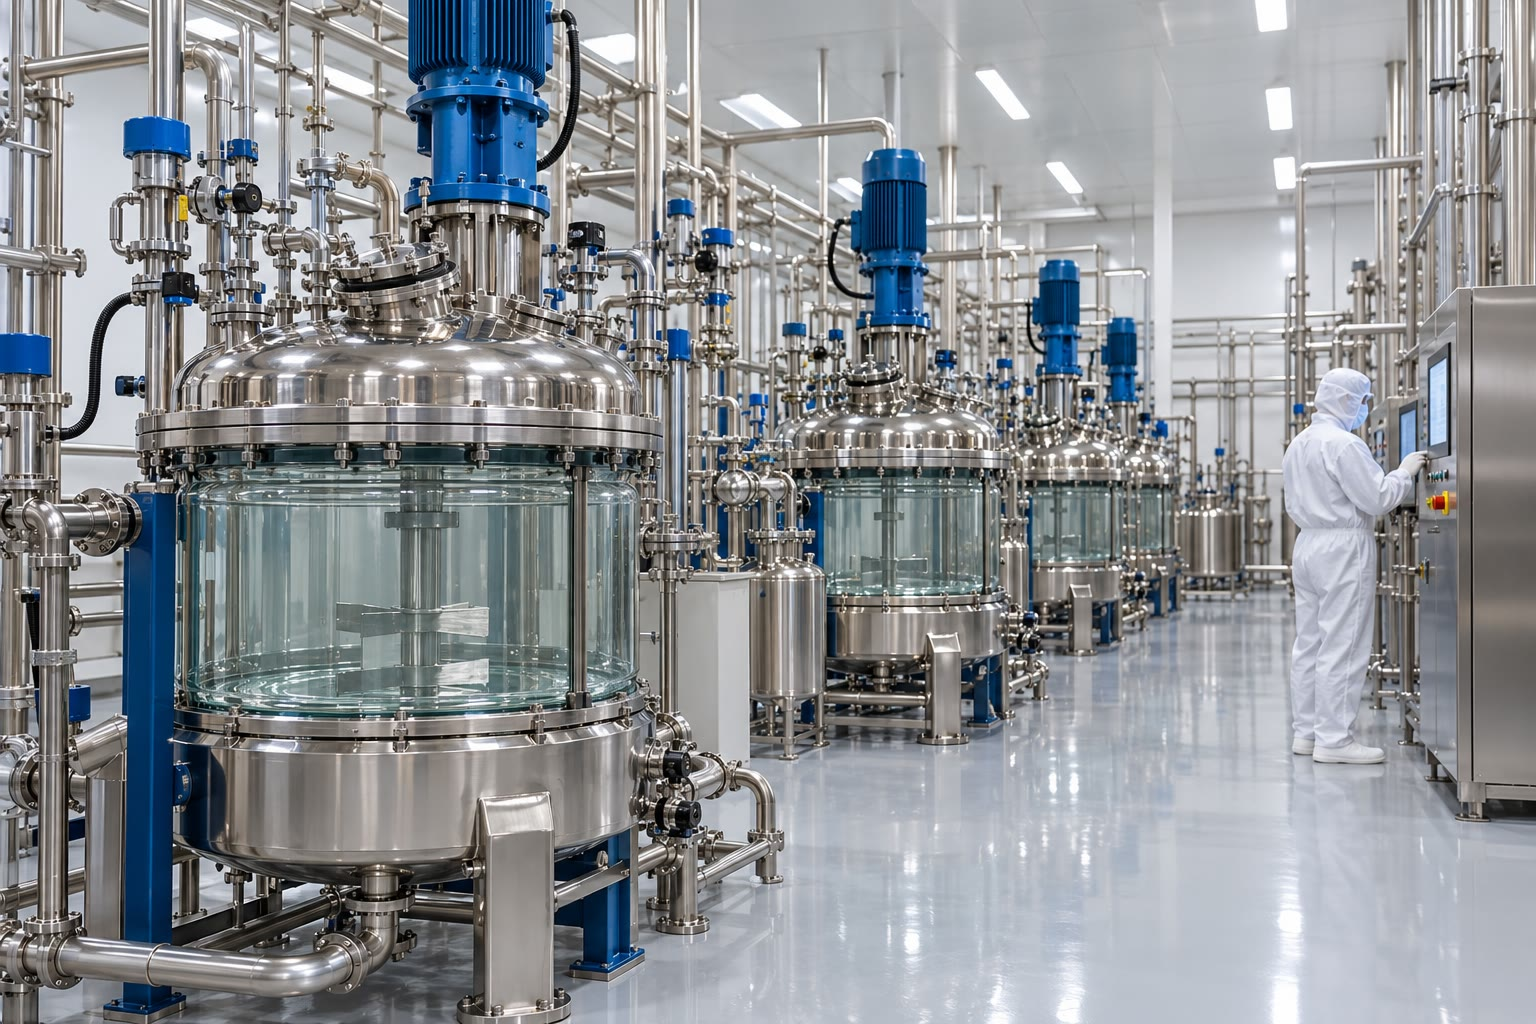
\includegraphics[width=0.58\linewidth]{images/book4/ai/b3-28-api-plant.jpg}

{\small Een hal met geëmailleerde reactoren in een fabriek die werkzame
farmaceutische bestanddelen maakt. Veel van haar producten zijn
afzonderlijke enantiomeren, gemaakt door katalyse of \omterm{def:b3:asymmetric-synthesis:resolution}{racemaatsplitsing} en
gecontroleerd met chirale chromatografie.}
\end{omfigure}

\section{Enantiomere zuiverheid meten}

\begin{definition}[Enantiomere overmaat]\label{def:b3:asymmetric-synthesis:ee}
Voor een mengsel van enantiomeren in hoeveelheden $n_R \ge n_S$ is de
\emph{enantiomere overmaat}\index{enantiomere overmaat} $\mathrm{ee} = (n_R - n_S)/(n_R + n_S)$ en de
\emph{enantiomeerverhouding}\index{enantiomeerverhouding} $\mathrm{er} = n_R/n_S$; voor diastereomeren wordt de
\emph{diastereomere overmaat}\index{diastereomere overmaat} de op dezelfde
manier gedefinieerd. De \emph{optische zuiverheid}\index{optische zuiverheid}
is de verhouding van de specifieke draaiing van een monster tot die van
de zuivere enantiomeer.
\end{definition}

\begin{proposition}[ee en er]\label{prop:b3:asymmetric-synthesis:ee-er}
$\mathrm{ee} = (\mathrm{er} - 1)/(\mathrm{er} + 1)$ en $\mathrm{er} = (1 + \mathrm{ee})/(1 - \mathrm{ee})$.
\end{proposition}

\begin{proof}
Deel teller en noemer van $(n_R - n_S)/(n_R + n_S)$ door $n_S$; oplossen naar er geeft de
tweede vorm.
\end{proof}

Een ee van 90\,\% is een er van 95\,:\,5, een ee van 98\,\% een er van
99\,:\,1. De \omterm{def:b3:asymmetric-synthesis:ee}{optische zuiverheid} is alleen gelijk aan de ee als de
draaiing evenredig is met de samenstelling; onzuiverheden, het
oplosmiddel, concentratie-effecten en de kleine draaiingen van veel
verbindingen maken ze onbetrouwbaar, en men meet de ee door de
enantiomeren te scheiden.

\begin{method}[ee uit een chiraal chromatogram]\label{met:b3:asymmetric-synthesis:ee-chromatogram}
\begin{enumerate}
  \item Injecteer eerst het racemaat, om de twee pieken te identificeren
        en hun scheiding (basislijnscheiding) en gelijke oppervlakten te
        controleren.
  \item Injecteer het monster en integreer beide pieken.
  \item De enantiomeren hebben dezelfde respons in een achirale detector,
        zodat
        $\mathrm{ee} = (A_1 - A_2)/(A_1 + A_2)$; ken de pieken toe met een enantiozuivere standaard.
\end{enumerate}
\end{method}

\begin{omfigure}
\begin{tikzpicture}
\begin{axis}[name=a, width=0.48\linewidth, height=5.4cm, xmin=0, xmax=20, ymin=0, ymax=1.0,
  axis lines=left, xlabel={$\Delta\Delta G^\ddagger$ / \unit{kJ.mol^{-1}}}, ylabel={ee},
  tick label style={font=\scriptsize}, label style={font=\small}]
\addplot[omDef, thick] table[x=ddg, y=eeA] {figdata/out/bachelor-3-er-ddg.dat};
\addplot[omMeth, thick] table[x=ddg, y=eeB] {figdata/out/bachelor-3-er-ddg.dat};
\addplot[omThm, thick] table[x=ddg, y=eeC] {figdata/out/bachelor-3-er-ddg.dat};
\node[font=\scriptsize, omDef, anchor=west] at (axis cs:10,0.55) {\qty{-78}{\celsius}};
\node[font=\scriptsize, omMeth, anchor=west] at (axis cs:10,0.43) {\qty{0}{\celsius}};
\node[font=\scriptsize, omThm, anchor=west] at (axis cs:10,0.31) {\qty{25}{\celsius} (laagste kromme)};
\end{axis}
\begin{axis}[at={(a.east)}, anchor=west, xshift=1.4cm, width=0.48\linewidth, height=5.4cm,
  xmin=7.5, xmax=9.5, ymin=0, axis lines=left, ytick=\empty,
  xlabel={retentietijd / min}, ylabel={detectorsignaal},
  tick label style={font=\scriptsize}, label style={font=\small}]
\addplot[black, thick] table[x=t, y=y] {figdata/out/bachelor-3-er-ddg-b.dat};
\node[font=\scriptsize, anchor=south west] at (axis cs:8.3,250) {(\textit{R}): 97.5};
\node[font=\scriptsize, anchor=south] at (axis cs:9.1,20) {(\textit{S}): 2.5};
\end{axis}
\end{tikzpicture}

{\small Links: \omterm{def:b3:asymmetric-synthesis:ee}{enantiomere overmaat} tegen het verschil in \omterm{def:b3:rate-theories:activation}{gibbsenergie van
activering} van de twee concurrerende wegen, bij drie temperaturen:
dezelfde
$\Delta\Delta G^\ddagger$ geeft een hogere ee bij lage temperatuur. Rechts: een chiraal HPLC-chromatogram,
piekoppervlakten 97.5 en 2.5 (model): ee 95\,\%.}
\end{omfigure}

NMR onderscheidt enantiomeren alleen in een chirale omgeving: een chiraal
solvatatiereagens vormt kortlevende diastereomere complexen waarvan de
signalen verschillen, en een chirale alcohol of een chiraal amine,
omgezet in zijn twee diastereomere esters met het zuur van Mosher, toont
de configuratie via het patroon van de verschuivingsverschillen.

\begin{method}[Configuratie uit mosheresters, in grote lijnen]\label{met:b3:asymmetric-synthesis:mosher}
\begin{enumerate}
  \item Maak zowel de (\textit{R})- als de (\textit{S})-MTPA-ester van de alcohol.
  \item Neem hun protonspectra op en bereken $\Delta\delta = \delta_S - \delta_R$ voor de protonen aan elke
        kant van het carbinolkoolstofatoom.
  \item In de voorkeursconformatie schermt de fenylring van het zuur één
        kant af:
        protonen met $\Delta\delta > 0$ liggen aan de ene kant, die met $\Delta\delta < 0$ aan de andere, wat
        de twee substituenten plaatst en de configuratie geeft.
\end{enumerate}
\end{method}

\section{Topiciteit en stereoselectieve addities}

\begin{definition}[Stereoselectieve reacties]\label{def:b3:asymmetric-synthesis:selective}
Een \emph{enantioselectieve reactie}\index{enantioselectieve reactie} vormt
de ene enantiomeer van een product in overmaat ten opzichte van de
andere; een \emph{diastereoselectieve
reactie}\index{diastereoselectieve reactie} vormt één diastereomeer in
overmaat.
\end{definition}

\begin{definition}[Topiciteit]\label{def:b3:asymmetric-synthesis:topicity}
Twee groepen van een molecuul zijn \emph{homotoop}\index{homotoop} als ze
verwisseld worden door een rotatie van het molecuul (de vervanging van
elk van beide geeft dezelfde verbinding),
\emph{enantiotoop}\index{enantiotoop} als ze alleen door een spiegeling
verwisseld worden (de vervanging van de ene of de andere geeft
enantiomeren), en
\emph{diastereotoop}\index{diastereotoop} als geen enkele
\omterm{def:b3:point-groups:operation}{symmetrieoperatie} ze verwisselt (de vervanging van de ene of de andere
geeft diastereomeren).
\end{definition}

De twee waterstofatomen van een groep $\ce{CH2}$ naast een stereocentrum zijn \omterm{def:b3:asymmetric-synthesis:topicity}{diastereotoop}: ze
hebben verschillende chemische verschuivingen en koppelen met elkaar,
waardoor zo'n groep in NMR vaak als twee signalen verschijnt.

\begin{definition}[Prochirale vlakken]\label{def:b3:asymmetric-synthesis:faces}
Een trigonaal koolstofatoom met drie verschillende substituenten is
\emph{prochiraal}\index{prochiraal}: additie van een vierde, verschillende
groep maakt een stereocentrum. Het vlak waarop de drie substituenten in
dalende CIP-prioriteit met de klok mee lopen, is het
\emph{Re-vlak}\index{Re-vlak}; tegen de klok in, het
\emph{Si-vlak}\index{Si-vlak}.
\end{definition}

\begin{omfigure}
\begin{tikzpicture}[font=\small, >=Stealth]
  \coordinate (c) at (0,0);
  \draw[thick, double, double distance=1.6pt] (c) -- (90:1.1) node[above] {O (1)};
  \draw[thick] (c) -- (210:1.1) node[below left] {$\ce{C6H5}$ (2)};
  \draw[thick] (c) -- (330:1.1) node[below right] {$\ce{CH3}$ (3)};
  \fill (c) circle (1.6pt);
  \draw[->, thick, omThm] (70:0.6) arc[start angle=70, end angle=200, radius=0.6];
  \node[font=\scriptsize, omThm, align=center] at (-1.9,0.75) {1 $\to$ 2 $\to$ 3\\ tegen de klok in:\\ \textit{Si}-vlak};
  \node[font=\scriptsize, align=left, anchor=west] at (2.6,0.4) {vlak naar de lezer: \textit{Si}\\ vlak achter het blad: \textit{Re}};
  \node[font=\scriptsize, align=left, anchor=west] at (2.6,-0.5) {hydride, toegevoegd vanaf het \textit{Re}-vlak,\\ geeft (\textit{S})-1-fenylethanol};
\end{tikzpicture}

{\small De vlakken van acetofenon. Van voren gezien lopen de substituenten
van het carbonylkoolstofatoom in CIP-volgorde (O, fenyl, methyl) tegen de
klok in: het voorvlak is \textit{Si}, het achtervlak \textit{Re}.}
\end{omfigure}

\begin{method}[Re- en Si-vlakken toekennen]\label{met:b3:asymmetric-synthesis:re-si}
\begin{enumerate}
  \item Rangschik de drie substituenten van het trigonale atoom volgens de
        regels van CIP (een dubbele binding telt haar partner twee keer).
  \item Kijk naar het betrokken vlak, met het trigonale vlak in het vlak
        van het blad.
  \item Met de klok mee 1 $\to$ 2 $\to$ 3: \textit{Re}; tegen de klok in: \textit{Si}.
  \item Om het product te benoemen, voeg je de nieuwe groep naar de
        kijker toe en pas je de regels van CIP toe op het nieuwe
        stereocentrum; een aanval op Re geeft niet altijd \textit{R}.
\end{enumerate}
\end{method}

\begin{definition}[Model van Felkin-Anh en chelatiecontrole]\label{def:b3:asymmetric-synthesis:felkin}
Het \emph{model van Felkin-Anh}\index{model van Felkin-Anh} voorspelt de
belangrijkste diastereomeer van een nucleofiele additie aan een
carbonylgroep naast een stereocentrum: de grootste groep op dat centrum
staat loodrecht op het carbonylvlak, en het nucleofiel nadert anti ten
opzichte ervan, langs de kleinste groep, volgens het traject van
Bürgi-Dunitz. Bij
\emph{chelatiecontrole}\index{chelatiecontrole} vergrendelt een metaalion
dat zowel aan het carbonylzuurstofatoom als aan een donorgroep op het
stereocentrum gebonden is de conformatie, en addeert het nucleofiel aan
het minst gehinderde vlak van de chelaatring.
\end{definition}

\begin{proposition}[Selectiviteit volgens Felkin-Anh]\label{prop:b3:asymmetric-synthesis:felkin}
Voor een $\alpha$-chiraal aldehyde of keton zonder chelerende groep is het
belangrijkste product dat wat het \omterm{def:b3:asymmetric-synthesis:felkin}{model van Felkin-Anh} voorspelt (een
empirisch model, ondersteund door berekeningen). \admitted
\end{proposition}

\begin{omfigure}
\begin{tikzpicture}[font=\small, >=Stealth]
  \foreach \a/\lab in {90/L, 330/M, 210/S} {
    \draw[line width=0.8pt] (\a:0.55) -- (\a:1.1) node[pos=1.3] {\lab};
  }
  \fill[white] (0,0) circle (0.55);
  \draw[line width=0.8pt] (0,0) circle (0.55);
  \draw[line width=0.8pt, double, double distance=1.4pt] (0,0) -- (0:1.1) node[right] {O};
  \draw[line width=0.8pt] (0,0) -- (180:1.1) node[left] {R};
  \draw[->, very thick, omThm] (250:2.2) -- (250:0.25);
  \node[omThm, anchor=north] at (250:2.25) {Nu$^-$};
  \node[font=\scriptsize, align=left, anchor=west] at (1.7,-1.0) {Nu$^-$ komt binnen anti t.o.v.\ L,\\ langs S, onder ongeveer 107°\\ met de binding C=O};
\end{tikzpicture}

{\small \omterm{def:b3:asymmetric-synthesis:felkin}{Model van Felkin-Anh}, gezien langs de binding van het
carbonylkoolstofatoom (voor, met bindingen naar O en R) naar het
stereocentrum (achterste cirkel, groepen L, M en S). De grote groep staat
loodrecht op het carbonylvlak; het nucleofiel komt van de andere kant,
dicht bij de kleine groep en weg van het zuurstofatoom.}
\end{omfigure}

\section{Strategieën}

\begin{definition}[Chirale pool]\label{def:b3:asymmetric-synthesis:chiral-pool}
De \emph{chirale pool}\index{chirale pool} is de verzameling goedkope,
enantiozuivere natuurlijke verbindingen (aminozuren, suikers, terpenen,
hydroxyzuren) die als uitgangsstoffen gebruikt worden, waarbij hun
stereocentra in het doelmolecuul terechtkomen.
\end{definition}

\begin{definition}[Chirale hulpgroep]\label{def:b3:asymmetric-synthesis:auxiliary}
Een \emph{chirale hulpgroep}\index{chirale hulpgroep} is een enantiozuivere
groep die tijdelijk aan een substraat gekoppeld wordt om de stereochemie
van een reactie te sturen, en daarna verwijderd en teruggewonnen wordt.
\end{definition}

Bij de alkyleringen van Evans wordt een oxazolidinon, gemaakt uit een
aminozuur, geacyleerd; het lithium- of natriumenolaat, gechelateerd aan
de carbonylgroep van de hulpgroep, wordt door een alkylhalogenide
aangevallen aan het vlak dat van de substituent van de hulpgroep
afgekeerd is, wat één diastereomeer geeft, vaak met een de boven
95\,\%; hydrolyse maakt daarna het chirale zuur en de hulpgroep vrij.

\begin{definition}[Racemaatsplitsingen]\label{def:b3:asymmetric-synthesis:resolution}
De \emph{racemaatsplitsing}\index{racemaatsplitsing} is de scheiding van
een racemaat in zijn enantiomeren, klassiek door diastereomere zouten met
een enantiozuiver zuur of een enantiozuivere base te kristalliseren. Bij
een \emph{kinetische racemaatsplitsing}\index{kinetische racemaatsplitsing}
reageren de twee enantiomeren met verschillende snelheden met een chiraal
reagens of een chirale katalysator, met selectiviteit $s = k_{\mathrm{snel}}/k_{\mathrm{traag}}$. Bij een
\emph{dynamische kinetische
racemaatsplitsing}\index{dynamische kinetische racemaatsplitsing} gaan de
enantiomeren van het substraat snel in elkaar over terwijl een van beide
reageert.
\end{definition}

\begin{theorem}[Vergelijking van Kagan]\label{thm:b3:asymmetric-synthesis:kagan}
Bij een \omterm{def:b3:asymmetric-synthesis:resolution}{kinetische racemaatsplitsing} van een racemaat door reacties van de eerste orde met selectiviteit $s$
zijn de omzetting $c$ en de ee van het resterende substraat verbonden door
\[
  s = \frac{\ln[(1 - c)(1 - \mathrm{ee})]}{\ln[(1 - c)(1 + \mathrm{ee})]}.
\]
\end{theorem}

\begin{proof}
Elke enantiomeer neemt exponentieel af: de resterende fracties zijn $f_1 = \eu^{-k_{\mathrm{snel}}t}$ en
$f_2 = \eu^{-k_{\mathrm{traag}}t}$, dus $\ln f_1 = s\ln f_2$. Vertrekkend van gelijke hoeveelheden is $1 - c = (f_1 + f_2)/2$ en
$\mathrm{ee} = (f_2 - f_1)/(f_1 + f_2)$. Dan is $(1 - c)(1 - \mathrm{ee}) = \tfrac12(f_1 + f_2)\cdot 2f_1/(f_1 + f_2) = f_1$ en evenzo
$(1 - c)(1 + \mathrm{ee}) = f_2$. Dus is $s = \ln f_1/\ln f_2$ de opgegeven verhouding.
\end{proof}

\begin{omfigure}
\begin{tikzpicture}
\begin{axis}[width=0.62\linewidth, height=5.6cm, xmin=0, xmax=1, ymin=0, ymax=1.02,
  axis lines=left, xlabel={omzetting $c$}, ylabel={ee},
  tick label style={font=\scriptsize}, label style={font=\small},
  legend style={font=\scriptsize, draw=none, at={(1.04,0.5)}, anchor=west}, legend cell align=left]
\addplot[color=omThm, thick] table[x=c, y=eesm] {figdata/out/bachelor-3-kinetic-resolution-s2.dat};
\addlegendentry{$s = 2$}
\addplot[color=omMeth, thick] table[x=c, y=eesm] {figdata/out/bachelor-3-kinetic-resolution-s10.dat};
\addlegendentry{$s = 10$}
\addplot[color=omDef, thick] table[x=c, y=eesm] {figdata/out/bachelor-3-kinetic-resolution-s50.dat};
\addlegendentry{$s = 50$}
\addplot[color=omThm, thick, dashed] table[x=c, y=eep] {figdata/out/bachelor-3-kinetic-resolution-s2.dat};
\addplot[color=omMeth, thick, dashed] table[x=c, y=eep] {figdata/out/bachelor-3-kinetic-resolution-s10.dat};
\addplot[color=omDef, thick, dashed] table[x=c, y=eep] {figdata/out/bachelor-3-kinetic-resolution-s50.dat};
\end{axis}
\end{tikzpicture}

{\small \omterm{def:b3:asymmetric-synthesis:resolution}{Kinetische racemaatsplitsing}: ee van het resterende substraat
(volle lijn) en van het product (gestreept) tegen de omzetting, voor drie
selectiviteiten. Het substraat kan altijd enantiozuiver gemaakt worden
door ver genoeg te gaan, ten koste van het rendement; het product is het
zuiverst bij lage omzetting.}
\end{omfigure}

\begin{proposition}[Dynamische kinetische racemaatsplitsing]\label{prop:b3:asymmetric-synthesis:dkr}
Als de enantiomeren van het substraat veel sneller in elkaar overgaan dan
elk van beide reageert, kan het hele racemaat omgezet worden in één
productenantiomeer, met een ee die bepaald wordt door $s$:
$\mathrm{er} = s$.
\end{proposition}

\begin{proof}
Een snelle racemisatie houdt de twee enantiomeren van het substraat op
elk ogenblik in gelijke hoeveelheden. De producten ontstaan dan met
snelheden in de verhouding $k_{\mathrm{snel}}[\mathrm A] : k_{\mathrm{traag}}[\mathrm A] = s$, en niets
houdt de reactie tegen voordat al het substraat, vooral via de snelle
enantiomeer, verbruikt is: het rendement kan 100\,\% bereiken met $\mathrm{er} = s$.
\end{proof}

\begin{method}[Een strategie kiezen]\label{met:b3:asymmetric-synthesis:strategy}
\begin{enumerate}
  \item Als de stereocentra van het doelmolecuul in een goedkope
        natuurlijke verbinding bestaan, vertrek je van de \omterm{def:b3:asymmetric-synthesis:chiral-pool}{chirale pool}.
  \item Gebruik voor een eenmalige synthese, of om een centrum
        betrouwbaar naast een carbonylgroep te plaatsen, een hulpgroep,
        ten koste van twee extra stappen.
  \item Als het racemaat goedkoop is en de ongewenste enantiomeer
        gerecycleerd of geracemiseerd kan worden, splits het dan
        (klassiek, kinetisch of dynamisch).
  \item Zoek op grote schaal een asymmetrische katalysator: één
        stereocentrum per katalytische cyclus, geen stoichiometrisch
        chiraal afval.
\end{enumerate}
\end{method}

\section{Asymmetrische katalyse met metalen}

\begin{definition}[Asymmetrische katalyse]\label{def:b3:asymmetric-synthesis:asymmetric-catalysis}
\emph{Asymmetrische katalyse}\index{asymmetrische katalyse} is
enantioselectieve synthese met een chirale katalysator die in kleine
hoeveelheid gebruikt wordt; bij metaalkatalysatoren komt de chiraliteit
meestal van een \emph{chiraal ligand}\index{chiraal ligand}.
\end{definition}

\begin{theorem}[Selectiviteit uit energie]\label{thm:b3:asymmetric-synthesis:er-ddg}
Als twee enantiomere producten via diastereomere overgangstoestanden met
gelijke pre-exponentiële factoren gevormd worden, onomkeerbaar en onder
kinetische controle, is
$\mathrm{er} = \exp(\Delta\Delta G^\ddagger/RT)$, waarin $\Delta\Delta G^\ddagger$ het verschil is van hun gibbsenergieën van
activering.
\end{theorem}

\begin{proof}
Volgens de \omterm{thm:b3:rate-theories:eyring}{vergelijking van Eyring} (\cref{ch:b3:rate-theories}) is
$k_i = (k_BT/h)\eu^{-\Delta G_i^\ddagger/RT}$; beide producten ontstaan uit dezelfde beginstoffen, zodat hun
snelheden op elk ogenblik in de verhouding $k_1/k_2 = \eu^{(\Delta G_2^\ddagger - \Delta G_1^\ddagger)/RT}$ staan, en de gevormde hoeveelheden ook.
\end{proof}

Bij \qty{25}{\celsius} vereist een ee van 99\,\% (er 199) een $\Delta\Delta G^\ddagger = RT\ln 199 = \qty{13.1}{kJ/mol}$, ongeveer de energie van één
waterstofbrug; bij \qty{-78}{\celsius} volstaat \qty{8.6}{kJ/mol}.

\begin{proposition}[Liganden met symmetrie $C_2$]\label{prop:b3:asymmetric-synthesis:c2}
Een \omterm{def:b3:asymmetric-synthesis:asymmetric-catalysis}{chiraal ligand} met symmetrie $C_2$ halveert het aantal diastereomere
overgangstoestanden dat vergeleken moet worden, omdat de twee
coördinatieplaatsen die het vrijlaat gelijkwaardig zijn.
\end{proposition}

\begin{proof}
De rotatie $C_2$ van de katalysator beeldt de ene vrije plaats af op de andere en laat de
katalysator ongewijzigd; elke overgangstoestand op de ene plaats is dus
identiek aan de gedraaide op de andere. Alleen de bindingswijzen op één
plaats (vlak van het substraat, oriëntatie) moeten vergeleken worden.
\end{proof}

Knowles gebruikte chirale monofosfines, daarna het difosfine DIPAMP met symmetrie $C_2$, met rodium om
een enamide te hydrogeneren tot het beschermde aminozuur van L-DOPA; het
BINAP van Noyori hydrogeneert met ruthenium ketonen en
gefunctionaliseerde alkenen, en, gecombineerd met een chiraal diamine,
eenvoudige ketonen met een zeer hoge ee. Bij de hydrogenering van
enamiden met rodium komt het belangrijkste product van het minder
stabiele, minoritaire complex van katalysator en substraat, dat veel
sneller met waterstof reageert: de selectiviteit wordt bepaald in de
overgangstoestanden, niet door de populaties van de intermediairen (het
principe van Curtin-Hammett).

\begin{definition}[Sharplessepoxidatie]\label{def:b3:asymmetric-synthesis:sharpless}
De \emph{sharplessepoxidatie}\index{sharplessepoxidatie} is de
enantioselectieve epoxidatie van allylalcoholen door \textit{tert}-butylhydroperoxide,
gekatalyseerd door titaan(IV)isopropoxide met een enantiozuiver
diethyltartraat; de alcohol bindt aan titaan, dat het zuurstofatoom
aflevert aan één vlak van het alkeen, gekozen door het tartraat.
\end{definition}

\begin{omfigure}
\begin{tikzpicture}[font=\small, >=Stealth]
  \draw[black!50] (-2.3,-1.55) rectangle (2.5,1.55);
  % C3 (top) = C2 (bottom); C2 carries R1 (left) and CH2OH (lower right),
  % C3 carries R2 (left) and R3 (right)
  \coordinate (c3) at (0,0.45); \coordinate (c2) at (0,-0.45);
  \draw[thick, double, double distance=1.6pt] (c3) -- (c2);
  \draw[thick] (c3) -- (-0.9,0.95) node[above left, inner sep=1pt] {R$^2$};
  \draw[thick] (c3) -- (0.9,0.95) node[above right, inner sep=1pt] {R$^3$};
  \draw[thick] (c2) -- (-0.9,-0.95) node[below left, inner sep=1pt] {R$^1$};
  \draw[thick] (c2) -- (0.9,-0.95) node[below right, inner sep=1pt] {$\ce{CH2OH}$};
  \draw[->, very thick, omDef] (0.35,2.5) -- (0.2,0.1) node[pos=0, above, align=center, font=\scriptsize] {D-($-$)-diethyltartraat:\\ O vanaf het bovenvlak};
  \draw[->, very thick, omThm] (0.35,-2.6) -- (0.2,-0.1) node[pos=0, below, align=center, font=\scriptsize] {L-($+$)-diethyltartraat:\\ O vanaf het ondervlak};
\end{tikzpicture}

{\small Het ezelsbruggetje van Sharpless. Met de allylalcohol in het vlak
getekend, de groep
$\ce{CH2OH}$ rechtsonder, levert L-($+$)-diethyltartraat het zuurstofatoom af van
onder het vlak en D-($-$)-diethyltartraat van erboven, wat de
substituenten $\mathrm R^1$ tot $\mathrm R^3$ ook zijn.}
\end{omfigure}

Hetzelfde idee, een metaal dat door een goedkoop natuurlijk ligand in een
chirale holte gehouden wordt, geeft de asymmetrische dihydroxylering van
alkenen volgens Sharpless met osmium en kinaalkaloïden als liganden. Als
het ligand niet enantiozuiver is, hoeft de ee van het product niet
evenredig te zijn met die van het ligand: aggregaten van twee liganden,
met verschillende activiteiten voor homochirale en heterochirale paren,
geven niet-lineaire effecten, soms nuttige versterkingen.

\section{Organokatalyse}

\begin{definition}[Organokatalyse]\label{def:b3:asymmetric-synthesis:organocatalysis}
\emph{Organokatalyse}\index{organokatalyse} is katalyse door kleine
organische moleculen zonder metalen. Bij
\emph{enaminekatalyse}\index{enaminekatalyse} zet een secundair amine een
keton of aldehyde om in een nucleofiel enamine; bij
\emph{iminiumkatalyse}\index{iminiumkatalyse} zet het een $\alpha,\beta$-onverzadigd
aldehyde om in een elektrofiel iminiumion met een verlaagde LUMO.
\end{definition}

\begin{omfigure}
\begin{tikzpicture}[font=\small]
  % proline-derived enamine and the aldehyde held by the carboxylic acid
  \coordinate (n) at (0,0.7); \coordinate (r2) at (0.67,0.22); \coordinate (r3) at (0.41,-0.57);
  \coordinate (r4) at (-0.41,-0.57); \coordinate (r5) at (-0.67,0.22);
  \draw[thick] (n) -- (r2) -- (r3) -- (r4) -- (r5) -- (n);
  \node[fill=white, inner sep=0.6pt] at (n) {N};
  \coordinate (ca) at (0,1.45); \coordinate (cb) at (0.72,1.85);
  \draw[thick] (0,0.88) -- (ca);
  \draw[thick] (ca) -- (-0.62,1.85) node[left, inner sep=1pt] {$\ce{CH3}$};
  \draw[thick, double, double distance=1.5pt] (ca) -- (cb);
  \coordinate (cacid) at (1.45,0.45);
  \draw[thick] (r2) -- (cacid);
  \draw[thick, double, double distance=1.5pt] (cacid) -- (1.75,-0.15) node[below, inner sep=1pt] {O};
  \draw[thick] (cacid) -- (2.05,0.9) node[right, inner sep=1pt] (oh) {O--H};
  \node (cald) at (1.55,2.55) {C};
  \draw[thick, double, double distance=1.5pt] (cald) -- (2.35,2.15) node[right, inner sep=1pt] (oald) {O};
  \draw[thick] (cald) -- (1.3,3.15) node[above, inner sep=1pt] {R};
  \draw[omThm, thick, densely dashed] (cb) -- (cald);
  \draw[omMeth, thick, dotted] (2.45,1.05) -- (2.5,2.0);
  \node[font=\scriptsize, omThm, anchor=east] at (1.05,2.35) {C--C vormt zich};
  \node[font=\scriptsize, omMeth, anchor=west] at (2.6,1.55) {H-brug};
\end{tikzpicture}

{\small De door proline gekatalyseerde aldolreactie, schematische
overgangstoestand: het enamine, gevormd uit aceton en het
pyrrolidinestikstofatoom, valt het aldehyde aan, waarvan het
zuurstofatoom door een waterstofbrug aan het carbonzuur van de
katalysator vastgehouden wordt; die brug legt vast welk vlak van het
aldehyde aangevallen wordt.}
\end{omfigure}

Proline, een goedkoop aminozuur, katalyseert intramoleculaire
aldolreacties van triketonen met een hoge ee (de ketonen van
Hajos-Parrish en Wieland-Miescher, sinds de jaren 1970 gebruikt voor
steroïdsyntheses) en, zoals in 2000 aangetoond, intermoleculaire
aldolreacties van aceton met aldehyden. Chirale imidazolidinonen werken
via iminiumionen in diels-alderreacties en geconjugeerde addities; chirale
fosforzuren, sterke brønstedzuren met een chirale holte, activeren imines
door protonering. Organokatalysatoren zijn stabiel tegenover lucht en
water en laten geen metaal in het product achter.

\begin{inthelab}[Een chirale HPLC-analyse]
Een chirale kolom, silica bekleed met een cellulose- of
amylosederivaat, wordt in evenwicht gebracht met een mengsel van hexaan
en isopropanol. Eerst wordt het racemaat geïnjecteerd en de
oplosmiddelverhouding bijgesteld tot de twee pieken tot op de basislijn
gescheiden zijn; daarna wordt het monster, opgelost in het eluens bij
ongeveer een milligram per milliliter, geïnjecteerd, en worden de pieken
geïntegreerd bij een golflengte waar beide absorberen.
\end{inthelab}

\begin{safety}{\ghs[0.6cm]{GHS02}\ghs[0.6cm]{GHS05}\ghs[0.6cm]{GHS06}\ghs[0.6cm]{GHS08}\ghs[0.6cm]{GHS09}}
% ledger: ghs4:TBHP, ghs4:TiOiPr4
\textit{tert}-Butylhydroperoxide: ontvlambaar, zelfontledend bij
verhitting, giftig bij contact met de huid, bijtend, sensibiliserend,
verdacht van het veroorzaken van genetische defecten; het wordt als
oplossing gebruikt, koel bewaard, nooit geconcentreerd, en overtollig
peroxide wordt vóór de opwerking vernietigd. Titaan(IV)isopropoxide:
ontvlambaar, irriterend, ontleed door vocht.
\end{safety}

\begin{history}[Twee prijzen voor asymmetrische katalyse]
William Knowles, Ryoji Noyori en Barry Sharpless deelden de Nobelprijs
voor de Scheikunde van 2001 voor chiraal gekatalyseerde hydrogeneringen
en oxidaties. Benjamin List en David MacMillan, die in 2000 aangetoond
hadden dat kleine organische moleculen \omterm{def:b3:asymmetric-synthesis:selective}{enantioselectieve reacties} even
breed konden katalyseren als metaalcomplexen, ontvingen de prijs van
2021.
\end{history}

\section{Oefeningen}

\begin{exercise}[$\star$]\label{exo:b3:asymmetric-synthesis:1}
Zet om: ee 80\,\% naar er; er 99\,:\,1 naar ee; ee 50\,\% naar het
percentage van elke enantiomeer.
\end{exercise}

\begin{exercise}[$\star$]\label{exo:b3:asymmetric-synthesis:2}
Een chiraal HPLC-chromatogram toont voor de twee enantiomeren pieken met
oppervlakten 1840 en 60. Bereken de ee.
\end{exercise}

\begin{exercise}[$\star$]\label{exo:b3:asymmetric-synthesis:3}
Ken het Re- en het \omterm{def:b3:asymmetric-synthesis:faces}{Si-vlak} toe van het carbonylkoolstofatoom van
propanal, en benoem de alcohol die ontstaat door additie van een
methylnucleofiel aan het \omterm{def:b3:asymmetric-synthesis:faces}{Re-vlak}.
\end{exercise}

\begin{exercise}[$\star$]\label{exo:b3:asymmetric-synthesis:4}
Zijn de twee methyleenprotonen van ethanol \omterm{def:b3:asymmetric-synthesis:topicity}{homotoop}, \omterm{def:b3:asymmetric-synthesis:topicity}{enantiotoop} of \omterm{def:b3:asymmetric-synthesis:topicity}{diastereotoop}?
En die van de groep $\ce{CH2}$ van 2-butanol?
\end{exercise}

\begin{exercise}[$\star\star$]\label{exo:b3:asymmetric-synthesis:5}
Bereken de $\Delta\Delta G^\ddagger$ die nodig is voor 99\,\% ee bij \qty{25}{\celsius} en bij \qty{-78}{\celsius}, en de ee die bij \qty{-78}{\celsius}
gegeven wordt door een katalysator die bij \qty{25}{\celsius} 80\,\% ee geeft (dezelfde $\Delta\Delta G^\ddagger$).
\end{exercise}

\begin{exercise}[$\star\star$]\label{exo:b3:asymmetric-synthesis:6}
Een monster van een amine heeft $[\alpha]_D = -12.0$ onder omstandigheden waarin de zuivere enantiomeer (\textit{S})
$-15.0$ heeft (gegevens van de oefening). Geef zijn \omterm{def:b3:asymmetric-synthesis:ee}{optische zuiverheid} en
de percentages van de enantiomeren, in de veronderstelling dat de
draaiing evenredig is met de samenstelling. Waarom is deze meting minder
betrouwbaar dan chromatografie?
\end{exercise}

\begin{exercise}[$\star\star$]\label{exo:b3:asymmetric-synthesis:7}
Bij een door lipase gekatalyseerde acetylering van een racemische
alcohol heeft de resterende alcohol bij 60\,\% omzetting een ee van
90\,\%. Bereken $s$.
\end{exercise}

\begin{exercise}[$\star\star$]\label{exo:b3:asymmetric-synthesis:8}
Voorspel het epoxide dat uit (\textit{E})-hex-2-een-1-ol ontstaat met L-($+$)-diethyltartraat, en met
D-($-$)-diethyltartraat.
\end{exercise}

\begin{exercise}[$\star\star$]\label{exo:b3:asymmetric-synthesis:9}
(\textit{S})-2-fenylpropanal wordt behandeld met methylmagnesiumbromide. Voorspel met het
\omterm{def:b3:asymmetric-synthesis:felkin}{model van Felkin-Anh} de belangrijkste diastereomeer.
\end{exercise}

\begin{exercise}[$\star\star\star$]\label{exo:b3:asymmetric-synthesis:10}
Toon aan dat bij een \omterm{def:b3:asymmetric-synthesis:resolution}{kinetische racemaatsplitsing} de ee van het product bij lage omzetting naar $(s - 1)/(s + 1)$
gaat, en bereken die voor $s = 20$. Waarom is een \omterm{def:b3:asymmetric-synthesis:resolution}{kinetische
racemaatsplitsing} beter om het substraat te zuiveren dan om het product
te maken?
\end{exercise}

\begin{exercise}[$\star\star\star$]\label{exo:b3:asymmetric-synthesis:11}
Een keton met een racemiseerbaar stereocentrum naast de carbonylgroep
wordt gereduceerd door een \omterm{def:b3:complex-kinetics:enzyme}{enzym} met $s = 99$, terwijl de racemisatie snel is. Welk
rendement en welke ee kunnen bereikt worden? Vergelijk met hetzelfde
\omterm{def:b3:complex-kinetics:enzyme}{enzym} zonder racemisatie, gestopt bij 50\,\% omzetting.
\end{exercise}

\begin{exercise}[$\star\star\star$]\label{exo:b3:asymmetric-synthesis:12}
Leg met het principe van Curtin-Hammett uit hoe het minoritaire complex
van katalysator en substraat het belangrijkste product kan geven, met
twee complexen in evenwicht
($K = 10$ in het voordeel van A) die reageren met $k_B/k_A = 600$.
\end{exercise}

\section{Probleem: de route naar L-DOPA}

\begin{problem}[{Weekendprobleem --- de route naar L-DOPA: het prochirale
enamide en zijn vlakken, de energie achter 95\,\% ee, zuivering door
kristallisatie, en wat een kinetische racemaatsplitsing nodig zou hebben
gehad}]
\label{pb:b3:asymmetric-synthesis:1}
% ledger: const:R
Gegevens van het probleem: de door rodium gekatalyseerde hydrogenering
van de enamideprecursor bij \qty{25}{\celsius} geeft het beschermde aminozuur (\textit{S}) met 95\,\% ee. Het ruwe
product, 100 g, wordt omgekristalliseerd: de moederloog houdt de hele
minoritaire enantiomeer vast en 5.0 g van de majoritaire.

\medskip\noindent\textbf{Deel I --- Het substraat.}
\begin{enumerate}
  \item Waarom is het enamide \omterm{def:b3:asymmetric-synthesis:faces}{prochiraal}? Welk koolstofatoom wordt een
        stereocentrum?
  \item Wat zou een achirale katalysator geven?
  \item Waarom is de amidegroep op het alkeen belangrijk voor de
        katalysator?
  \item Wat doet het chirale difosfine?
  \item Ontstaat het belangrijkste product uit het stabielere complex van
        katalysator en substraat?
  \item Waarom wordt de waterstof in elk complex maar aan één vlak
        toegevoegd?
\end{enumerate}

\medskip\noindent\textbf{Deel II --- Energie.}
\begin{enumerate}[resume]
  \item Geef de er voor 95\,\% ee.
  \item Bereken $\Delta\Delta G^\ddagger$ bij \qty{25}{\celsius}.
  \item Welke ee zou dezelfde $\Delta\Delta G^\ddagger$ geven bij \qty{-78}{\celsius}?
  \item Welke ee zou een $\Delta\Delta G^\ddagger$ die \qty{2}{kJ/mol} groter is, geven bij \qty{25}{\celsius}?
  \item Vergelijk \qty{9}{kJ/mol} met de energie van een waterstofbrug, en
        becommentarieer.
  \item Waarom laat men de reactie niet gewoon kouder verlopen?
\end{enumerate}

\medskip\noindent\textbf{Deel III --- Kristallisatie.}
\begin{enumerate}[resume]
  \item Bereken de massa's van de twee enantiomeren in het ruwe product.
  \item Bereken de massa en de ee van de kristallen.
  \item Bereken het rendement van de kristallisatie.
  \item Waarom kan kristallisatie de ee van een monster verhogen, maar
        haar nooit uit een racemaat scheppen (voor een verbinding die als
        racemische verbinding kristalliseert)?
  \item Hoe wordt de uiteindelijke ee gecontroleerd?
\end{enumerate}

\medskip\noindent\textbf{Deel IV --- In plaats daarvan een \omterm{def:b3:asymmetric-synthesis:resolution}{kinetische racemaatsplitsing}.}
\begin{enumerate}[resume]
  \item Wat is het maximale rendement aan één enantiomeer bij een
        eenvoudige \omterm{def:b3:asymmetric-synthesis:resolution}{kinetische racemaatsplitsing}?
  \item Bereken de $s$ die nodig is voor 95\,\% ee van het resterende substraat bij 55\,\% omzetting.
  \item Welk rendement aan dat substraat verkrijgt men?
  \item Hoe zou een \omterm{def:b3:asymmetric-synthesis:resolution}{dynamische kinetische racemaatsplitsing} het rendement
        veranderen?
  \item Waarom was asymmetrische hydrogenering de betere industriële
        keuze?
  \item Waarom moet het rodium uit het geneesmiddel verwijderd worden, en
        hoe wordt het gemeten?
  \item Formuleer het resultaat: de $\Delta\Delta G^\ddagger$ voor 95\,\% ee bij \qty{25}{\celsius}.
\end{enumerate}
\end{problem}
